\NeedsTeXFormat{LaTeX2e}[1995/06/01]  % ist die richtige LaTeX-version installiert?

\documentclass[ngerman]{article}    % Die Dokumentklasse legt ein 

\usepackage{a4}                % Paket fuer A4 Seitenformat
\usepackage[ngerman]{babel}    % deutsche Sonderzeichen z. b. Anfuehrungsstricht, Trennmuster, etc
\usepackage[T1]{fontenc}       % korrekte Darstellung vieler Akzente und Schriftzeichen, z. B. deutscher Umlaute und "ß"
%%\usepackage[latin1]{inputenc}  % Character-encoding des ASCII files (wichtig, wenn Umlaute direkt eingegeben werden)
\usepackage[utf8]{inputenc}
\usepackage[left=3cm,right=2.5cm,top=2.7cm,bottom=1cm,includeheadfoot,a4paper]{geometry}
\usepackage{epigraph}
                               % latin1 - für unixoide und auch Windowssysteme
							   % ansinew - für Windows
							   % applemac - für den Mac
							   % utf8 - eine Alternative für alle obigen Systeme.
\usepackage{glossaries}
\usepackage{acronym}
\usepackage{textcase}
\usepackage{multicol}
\usepackage[official]{eurosym}
\usepackage[per-mode=symbol, output-decimal-marker={,}]{siunitx} 
\usepackage{amsthm}
\usepackage[style=alphabetic-verb,hyperref]{biblatex}
\usepackage[breaklinks=true]{hyperref}
\usepackage[hyphenbreaks]{breakurl}
\usepackage{epsfig}  
\usepackage{import}
\usepackage{standalone}
\usepackage{pgfplots}
\pgfplotsset{compat=1.17}
\bibliography{PraktikumsberichtPE}
% Paket zum Einbinden von postscript Graphiken
%\usepackage{float}             % Hilfesmakros beim Positionieren von Graphiken
%\usepackage[small,bf]{caption} % figure title packages
%\usepackage{psfrag}            % replace text in postscript drawings with latex-code (does not work in pdfLaTeX!)
\usepackage{amsfonts}          % zusaetzliche mathematische Schrifttypen (z. B. \mathbb{})
\usepackage{amssymb}           % zusaetzliche mathematische Symbole
\usepackage{amsmath}           % hilfreiche mathematische Zusatzbefehler (z. B. \eqref{})

\DeclareMathOperator{\sgn}{sgn}

\usepackage{amsbsy}            % fette Griechische Zeichen im Mathemodus
\usepackage{cleveref}
\usepackage{placeins}
%\usepackage{exscale}           % correct scaling of integral- and summation symbols
%\usepackage{theorem}           % provides theorem environments
\usepackage{ifpdf}
\ifpdf
  \usepackage{epstopdf}
\fi
\usepackage{graphicx}
\usepackage{psfrag}
\usepackage{csquotes}
\usepackage{tikz}
\usetikzlibrary{shapes,arrows}
\usetikzlibrary{math}
\usetikzlibrary{positioning,fit,arrows.meta,backgrounds}
\usetikzlibrary{external}

%%%%%%%%%%%%%%%%%%%%%%%%%%%%%%%%%%%%%%%%%%%%%%%%%%%%%%%%%%%%%%%%%%%%%%%%%%%%%%%%%%%%%%%%%%%%%%%%%
%%  ein paar kleine Modifikationen am Format
%%%%%%%%%%%%%%%%%%%%%%%%%%%%%%%%%%%%%%%%%%%%%%%%%%%%%%%%%%%%%%%%%%%%%%%%%%%%%%%%%%%%%%%%%%%%%%%%%

\tikzstyle{block} = [draw, fill=gray!20, rectangle, 
    minimum height=3em, minimum width=4em, text width=4em, text centered]
\tikzstyle{sum} = [draw, fill=gray!0, circle, node distance=2cm]
\tikzstyle{dot} = [draw, fill=black, circle,scale=0.5 , node distance=2cm]
\tikzstyle{input} = [coordinate]
\tikzstyle{output} = [coordinate]
\tikzstyle{pinstyle} = [pin edge={to-,thin,black}]

%% Zeilenabstand: 1 1/2-zeilig   (1.3)
\renewcommand{\baselinestretch}{1.3}

\theoremstyle{definition}
\newtheorem{definition}{Definition}[section]
\newtheorem{korollar}{Korollar}
%% Absatzabstand
\parskip1.5ex

%% erste Zeile eines Absatzes nicht einruecken
\parindent0em

%% Seitenumbruchsteuerung, bei wenigen Zeilen nach Ueberschrift am Zeilenende
\def\condbreak#1{\vskip 0pt plus #1\pagebreak[3]\vskip 0pt plus -#1\relax}
\usepackage{array}

\newenvironment{conditions}
  {\par\vspace{\abovedisplayskip}\noindent\begin{tabular}{>{$}l<{$} @{${}={}$} l}}
  {\end{tabular}\par\vspace{\belowdisplayskip}}

%%%%%%%%%%%%%%%%%%%%%%%%%%%%%%%%%%%%%%%%%%%%%%%%%%%%%%%%%%%%%%%%%%%%%%%%%%%%%%%%%%%%%%%%%%%%%%%%%%
%% diese beiden Befehle definieren Titel und Autoren. Diese werden vom Befehl \maketitle ausgewertet
%%%%%%%%%%%%%%%%%%%%%%%%%%%%%%%%%%%%%%%%%%%%%%%%%%%%%%%%%%%%%%%%%%%%%%%%%%%%%%%%%%%%%%%%%%%%%%%%%%
\title{Praktikumsbericht\\ % neue Zeile
      Konzeptionierung eines adaptiven Regelansatzes für ACC-Systeme}
\author{Leonard Kämpf, \\
Westsächsische Hochschule Zwickau\\
Automatisiertes Fahren und Fahrerassistenzsysteme}   % Hier immer alle Autoren eintragen
\begin{document}

\begin{titlepage}
	\centering
	{\scshape\Large Praktikumsbericht\par}
	\vspace{1.5cm}
	{\huge\bfseries Lokaliserung eines 1:8 Fahrzeugmodells im Raum mithilfe von stationären Kameras\par}
	\vspace{2cm}
	{\LARGE\itshape Leonard Kämpf\par}
	\vspace{.3cm}
	{Matr.Nr. 41561\\Kraftfahrzeugtechnik \\ Vertiefung Kraftfahrzeugmechatronik}
	\vfill
	Betrieblicher Betreuer\par
	\vspace{3cm}
	\large{Professor Dr.-Ing.~Rick {Voßwinkel}}\\
	\small{Westsächsische Hochschule Zwickau}

 	\vfill

% Bottom of the page
	{\large 24. Juni 2024\par}
\end{titlepage}       % erstellt Dokument-Kopf mit Titel und Authoren wie oben definiert
\newpage
\tableofcontents         % erstellt Inhaltsverzeichnis (bei Bedarf auskommentieren)



\newpage
\section*{Symbolverzeichnis}
\begin{acronym}[MMM]
\setlength{\itemsep}{-\parsep}
\acro{C_i}[$\mathbf{C_i}$]{intrinsische Kameramatrix}
\acro{c_{x}}[$c_{x}$]{Verschiebung des Koordinatenursprungs der Pixelkoordinaten in X-Richtung}
\acro{c_{y}}[$c_{y}$]{Verschiebung des Koordinatenursprungs der Pixelkoordinaten in Y-Richtung}
\acro{f_{x}}[$f_{x}$]{Brennweite, Abstand der Linse zum Kamerasensor in X-Richtung}
\acro{f_{y}}[$f_{y}$]{Brennweite, Abstand der Linse zum Kamerasensor in Y-Richtung}
\acro{k_{1..3}}[$k_{1..3}$]{Stärken der radialen Verzerrung in Abhängigkeit zum Abstand eines Bildpunktes vom Zentrum}
\acro{P}[$\textbf{P}$]{Projektionsmatrix}
\acro{p_{1..2}}[$p_{1..2}$]{Stärken der tangentialen Verzerrung in Abhängigkeit zum Abstand eines Bildpunktes vom Zentrum}
\acro{p_{ij}}[$p_{ij}$]{Elemente der Projektionsmatrix}
\acro{q}[$q$]{Quaternion}
\acro{r}[$r$]{radialer Abstand eines Punktes zum optischen Zentrum}
\acro{r_{ij}}[$r_{ij}$]{Elemente der Rotationsmatrix zur Beschreibung der Orientierung der Kamera im Raum}
\acro{t_{xyz}}[$t_{xyz}$]{Komponenten des Translationsvektors zur Beschreibung der Position der Kamera im Raum zum Weltkoordinatensystem}
\acro{uv}[$u$, $v$]{Bildkoordinaten in Pixel}
\acro{utv}[$\tilde{u}$, $\tilde{v}$]{Bildkoordinaten in Pixel}
\acro{w}[$w$]{homogene Skalierungskomponente}
\acro{x_{r}}[$x_{r}$]{radiale Krümmung in X-Richtung}
\acro{x_{t}}[$x_{t}$]{tangentiale Krümmung in X-Richtung}
\acro{y_{r}}[$y_{r}$]{radiale Krümmung in Y-Richtung}
\acro{y_{t}}[$y_{t}$]{tangentiale Krümmung in Y-Richtung}

\end{acronym}
\newpage

\section{Vorstellung des Unternehmens}

Die Westsächsische Hochschule Zwickau (WHZ) bietet mit ihren spezialisierten Studiengängen und Forschungsinitiativen ein dynamisches Umfeld für die Forschung und Lehre im Bereich des autonomen Fahrens und der Fahrerassistenzsysteme. Die WHZ zeichnet sich durch einen praxisnahen Ansatz und enge Verbindungen zur Automobilindustrie aus, wodurch Studierende die Möglichkeit erhalten, zukunftsweisende Technologien in einem realitätsnahen Umfeld kennenzulernen und aktiv an ihrer Entwicklung teilzuhaben.

Im Fachbereich Kraftfahrzeugtechnik an der WHZ werden den Studierenden alle Grundlagen in den Bereichen Verbrennungsmotoren und Antriebstechnik, Karossierbau, Unfallanalyse und Instandhaltung, sowie Kraftfahrzeugmechatronik beigebracht. In modernen Laboren und auf einem speziellen Testgelände werden Projekte durchgeführt, die unterschiedliche Aspekte dieser Spezialisierungsrichtungen adressieren. Die Abteilung für autonomes Fahren und Fahrerassistenzsysteme legt hierbei einen besonderen Fokus auf die Entwicklung und Verbesserung von Sensoren wie Kameras und LiDAR-Systemen, die essenziell für die Wahrnehmung und Orientierung autonomer Fahrzeuge im Straßenverkehr sind. Durch die Kombination von Daten dieser Sensoren entwickeln Forschende Algorithmen zur Objekterkennung, -klassifizierung und -verfolgung, die für die sichere Navigation und Interaktion autonomer Fahrzeuge erforderlich sind.

Ein weiterer Schwerpunkt der Forschung und Lehre liegt in der Entwicklung und Implementierung von Fahrerassistenzsystemen (Advanced Driver Assistance Systems, ADAS). Diese Systeme stellen die Grundlage für höhere Automatisierungsstufen dar und sind für sicherheitskritische Funktionen wie Notbrems- und Spurhalteassistenten verantwortlich. Im Studium lernen die Studierenden, wie ADAS-Systeme die Verkehrssicherheit durch präventive und korrigierende Eingriffe erhöhen und auf welche Weise zukünftige Systeme schrittweise zu vollautonomen Fahrfunktionen weiterentwickelt werden können.

Das Curriculum der WHZ soll schrittweise erweitert werden, damit die Studierenden die Grundlagen der Mechatronik und Sensorik bis hin zu fortgeschrittenen Themen wie maschinellem Lernen und künstlicher Intelligenz für die Fahrzeugtechnik erlernen können. Der praktische Teil der Ausbildung wird durch zahlreiche Projekte und Praktika unterstützt, bei denen Studierende das Erlernte direkt anwenden können. Die enge Zusammenarbeit mit Unternehmen der Automobilbranche ermöglicht es der Hochschule, ihre Ausbildung an den Anforderungen der Industrie auszurichten und ihre Studierenden auf die Herausforderungen der Praxis vorzubereiten.

Die WHZ ist außerdem in mehrere Forschungsnetzwerke eingebunden und nimmt an Projekten auf nationaler und internationaler Ebene teil, um den Austausch mit anderen Hochschulen und Forschungseinrichtungen zu fördern. Dies schafft ein Umfeld, in dem innovative Ideen entstehen und umgesetzt werden können, und stärkt die Position der Hochschule als wichtigen Akteur im Bereich der Mobilität der Zukunft. So entwickelt sich die WHZ weiter um ihren Studierenden und Forschenden ideale Voraussetzungen zu gewährleisten, damit sie sich den Herausforderungen des autonomen Fahrens und der Fahrerassistenzsysteme annehmen und aktiv an der Entwicklung zukunftsweisender Mobilitätslösungen mitzuwirken zu können. 


\section{Aufgabenstellung}

Die seitens des Unternehmens gestellte Aufgabenstellung lautet: Es ist eine Methode zur präzisen Lokalisierung eines 1:8 Fahrzeugmodells im Raum zu ermöglichen und die Grundlage für zukünftige Automatisierungslösungen zu schaffen, sollen stationäre Kameras zur Positionsbestimmung eingesetzt werden. Dabei spielen Technologien wie ROS (Robot Operating System) und Apriltag Detection eine zentrale Rolle, um die Position des Fahrzeugs zuverlässig zu erfassen und zu verfolgen.

Die Entwicklung solcher Lösungen erfordert fundiertes Wissen in den Bereichen Bildverarbeitung und Systemintegration. Um diesen Anforderungen gerecht zu werden, sind eine umfangreiche Einarbeitung sowie die Nutzung von Tools wie Ubuntu, ROS 2 und Docker erforderlich. Parallel dazu wird eine eingehende Literaturrecherche zu Methoden der Bildverarbeitung durchgeführt, um das theoretische Wissen in der Praxis erfolgreich anzuwenden.

Aktuell liegt der Fokus darauf, die Lokalisierungsgenauigkeit zu validieren und das entwickelte System im praktischen Einsatz zu erproben. Das Ziel besteht darin, eine robuste und zuverlässige Lokalisierungsmethode zu entwickeln, die später als Basis für weiterführende Automatisierungsprozesse dienen kann. Die folgenden Teilaufgaben sind im Rahmen dieser Aufgabe umzusetzen:

\begin{itemize}
    \item Einarbeitung in Ubuntu, ROS, ROS 2, Docker und Apriltag Detection
    \item Literaturrecherche zum Thema Bildverarbeitung und deren Anwendungsmöglichkeiten
    \item Prototypische Umsetzung der Lokalisierung des Fahrzeugmodells mit stationären Kameras
    \item Validierung der Positionsbestimmung und Überprüfung der Genauigkeit
    \item Dokumentation und Erstellung eines Abschlussberichts
\end{itemize}

Die Entwicklung einer genauen Lokalisierung des Fahrzeugmodells ist ein entscheidender Schritt in der Verarbeitungskette zur vollständigen Automatisierung des Systems. Die erfassten Positionsdaten liefern wichtige Eingangsgrößen für nachgelagerte Systeme, die auf der Grundlage dieser Informationen weitergehende Steuerungssignale für das Fahrzeug generieren.




\newpage

\section{Problemstellung}

Das Thema Lokalisierung spielt eine zunehmend wichtige Rolle in der Entwicklung autonomer Systeme, insbesondere in der Robotik und Automobilindustrie. Automatisierte Fahrzeuge und mobile Roboter benötigen präzise Positionierungsinformationen, um sich sicher und effizient im Raum bewegen zu können. Diese Daten sind entscheidend für die Navigation, Hindernisvermeidung und Interaktion mit der Umgebung.

Ein zentraler Baustein für die Umsetzung automatisierter Systeme ist die exakte Positionsbestimmung von Fahrzeugen. Bei der Lokalisierung eines 1:8 Fahrzeugmodells mittels stationärer Kameras geht es darum, die genaue Position und Orientierung des Fahrzeugs im Raum zu ermitteln. Dies bildet die Grundlage für weitergehende Automatisierungsprozesse, wie die Pfadplanung und Steuerung. Die Positionsdaten werden durch visuelle Markierungen wie Apriltags erfasst und in Echtzeit verarbeitet, um das Fahrzeug in seiner Umgebung zu verfolgen.

Die Anforderungen an die Lokalisierung sind dabei vielfältig: Neben der reinen Positionsgenauigkeit spielt auch die Robustheit gegenüber Umwelteinflüssen und die Echtzeitfähigkeit eine zentrale Rolle. Ein Problem bei der Lokalisierung mit Kamerasystemen ist die Genauigkeit der Positionsbestimmung, die von Faktoren wie der Auflösung der Kameras und der Ausrichtung der Tags beeinflusst wird. In der \autoref{fig:ansatz2} wird der grundlegende Aufbau des Lokalisierungssystems dargestellt: Die stationären Kameras erfassen visuelle Markierungen (Apriltags) auf dem Fahrzeugmodell und berechnen daraus die Position im Raum. Die ermittelten Koordinaten können im Anschluss im ROS (Robot Operating System) von anderen Knotenpunkten (Nodes) verwendet werden. Dort werden sie durch entsprechende Algorithmen verarbeitet und beispielsweise zur Steuerung des Fahrzeugs genutzt.

Der Lokalisierungsalgorithmus basiert dabei auf einer Kombination aus Bildverarbeitungs- und Kalibrierungsmethoden. Die Kameras ermitteln die 2D-Position des Fahrzeuges anhand der Markierungen, wobei die Genauigkeit der Messung maßgeblich von der Kameraposition und der Qualität der Bildverarbeitung abhängt. Um eine möglichst präzise und stabile Lokalisierung zu gewährleisten, ist es notwendig, die Parameter des Systems zu optimieren und die Algorithmen regelmäßig zu validieren. Die ermittelten Positionsdaten werden als Eingangsgrößen für weiterführende Steuerungsalgorithmen genutzt, die für die Bewegung des Fahrzeugs verantwortlich sind.


\newpage
\section{Vorbereitung}

Die Kamerakalibrierung stellt einen essenziellen Schritt in der präzisen Detektion und Positionsbestimmung mithilfe von AprilTags dar. AprilTags sind visuelle Markierungen, die in verschiedenen Anwendungen zur Objekterkennung und Lokalisierung genutzt werden, insbesondere in der Robotik und autonomen Fahrzeugsteuerung. Eine zuverlässige und genaue Detektion dieser Markierungen ist jedoch direkt abhängig von der Genauigkeit der verwendeten Kameramodelle. Hier kommt die Kamerakalibrierung ins Spiel, da sie dazu dient, die systematischen Verzerrungen und mögliche Abweichungen der intrinsischen Parameter gegenüber den Werten aus dem Datenblatt der Kamera zu kompensieren.

Kameras unterliegen inhärenten geometrischen Verzerrungen, die durch die Beschaffenheit ihrer Optik entstehen. Besonders erwähnenswert sind die radiale Verzerrung, bei der Bildpunkte am Rand des Bildes stärker verzogen werden als diejenigen im Zentrum, und die tangentiale Verzerrung, die durch leicht schräg angeordnete Linsen entstehen kann. Diese Verzerrungen führen dazu, dass die in den Bildern dargestellten Objekte nicht mit ihren tatsächlichen räumlichen Positionen übereinstimmen. Ohne eine Kalibrierung der Kamera würde die AprilTag-Erkennung daher ungenaue Positionen und Orientierungen liefern, was die weitere Nutzung der Positionsdaten erheblich beeinträchtigen könnte.

Im Rahmen der Kamerakalibrierung werden die inneren Parameter der Kamera erfasst, darunter die Brennweite, welche die Sichtweite und die Vergrößerung der Kamera darstellt, die optische Mitte (principal point), welche die Koordinaten des Bildpunktes in Pixeln beschreibt an dem die optische Achse der Kamera den Bildsensor schneidet, die Schiefe der optischen Achse zum Sensor, sowie die bereits erwähnten Verzerrungsparameter, erfasst. Mithilfe dieser Parameter kann dann ein präzises Kameramodell erstellt werden, das die Verzerrungen kompensiert und eine korrekte Projektion von 3D-Punkten auf die Bildebene ermöglicht. Bei der Detektion von AprilTags sind diese Korrekturen von zentraler Bedeutung, da sie die Berechnung der Tag-Position und -Orientierung relativ zur Kamera wesentlich verbessern. Nur durch eine korrekte Kalibrierung können die Positionen der erkannten AprilTags im Raum präzise berechnet werden, was für Anwendungen, die eine hohe Genauigkeit erfordern, unerlässlich ist. \cite{daftry2013flexible}



\newpage

Die Darstellung der intrinsische Kameramatrix, sowie tangentialer und radialer Verzerrung in mathematischer Schreibweise nach \cite{Zhang2023} sehen wie folgt aus:

intrinsische Kameramatrix
\begin{equation}   
    \text{C}_i =  \begin{pmatrix} \text{f}_x & 0 & \text{c}_x \\ 0 & \text{f}_y & \text{c}_y \\ 0 & 0 & 1 \end{pmatrix}
\end{equation}

radiale Krümmung

\begin{equation}
    \begin{split}
    x_{r} =  x( 1 + k_1 r^2 + k_2 r^4 + k_3 r^6)  \\
    y_{r} = y( 1 + k_1 r^2 + k_2 r^4 + k_3 r^6)
    \end{split}
\end{equation}
tangentiale Krümmung
\begin{equation}
    \begin{split}
        x_{t} = x + [ 2p_1xy + p_2(r^2+2x^2)] \\
        y_{t} = y + [ p_1(r^2+ 2y^2)+ 2p_2xy]
    \end{split}
\end{equation}

Wobei \text{r} für den radialen Abstand des Bildpunktes zum optischen Zentrums steht und durch die Formel:
\begin{equation}
    r = \sqrt{x^2 + y^2}
\end{equation}

berechnet wird. 



Die Schätzung der intrinsischen Parameter einer Kamera kann durch bereits vorhandene Software-Tools von OpenCV oder MATLAB zuverlässig und präzise durchgeführt werden. Diese Tools nutzen zur Kalibrierung meist standardisierte Schachbrettmuster mit bekannten geometrischen Maßen. Die Kalibrierungssoftware erkennt dabei die Quadrate und inneren Eckpunkte des Schachbretts und verwendet diese, um die exakten Positionen der Objektpunkte im Raum zu bestimmen.

Anhand der bekannten Abstände zwischen den Ecken des Schachbrettmusters lassen sich die 3D-Koordinaten der Objektpunkte im Raum ermitteln. Durch eine Projektion dieser 3D-Punkte auf die 2D-Bildebene können die intrinsischen Parameter der Kamera, wie Brennweite, optische Mitte, sowie tangentiale und radiale Verzerrung geschätzt werden. Für eine hinreichende Kalibrierung der Kamera sind mindestens zehn Bilder erforderlich, da sich die Genauigkeit der Schätzung erfahrungsgemäß mit der Anzahl der aufgenommenen Bilder verbessert.

Um diese Voraussetzung zu erfüllen, wurde eine ROSbag-Datei erstellt und ein Python-Skript entwickelt, das einzelne Kameraframes aus der ROSbag extrahiert und im PNG-Format speichert. Die Auswahl der Bilder erfolgte gezielt: Nur solche Frames wurden verwendet, in denen das Schachbrettmuster eine veränderte Entfernung und/oder Ausrichtung zur Kamera aufweist. Dadurch konnte eine möglichst vielfältige Menge an Kalibrierungsbildern erzielt werden, um die Schätzung der intrinsischen Parameter weiter zu optimieren.


\newpage

In \autoref{tab:coeffi} sind alle Schätzwerte, welche aus der Kamerakalibrierung mithilfe von OpenCV resultierten aufgeführt, sowie Bilder vor und nach der Kamerakalibrierung. In \autoref{fig:vorkal} wird das Bild vor der Kamerakalibrierung gezeigt und in \autoref{fig:nachkal} nach der Kalibrierung. \\

\begin{table}[h]
    \centering
    \caption{Ergebnisse der Kamerakalibrierung mithilfe von OpenCV}
    \label{tab:coeffi}
    \begin{tabular}[h]{|l|c|l|l|}
    \hline
    \multicolumn{2}{|c|}{Parameter}  & \multicolumn{2}{c|}{Werte}  \\
    \hline
     $f_x$  & $c_x$ & $1,38105646 \cdot 10^{3}$ & $\text{$9,11397972 \cdot 10^{2}$}$\\
    \hline
     $f_y$  & $c_y$ &  $\text{$1,38624259 \cdot 10^{3}$}$  & $\text{$5,94349795 \cdot 10^{2}$}$\\
    \hline
     $k_1$ & $p_1$& $\text{0,0608873}$ & $\text{0,00066334}$\\
    \hline
     $k_2$ & $p_2$ & $\text{0,11741663}$ & $\text{0,0008057}$\\
    \hline
    \multicolumn{2}{|l|}{$k_3$} & \multicolumn{2}{l|}{$\text{-0,03352508}$} \\
    \hline
    
    \end{tabular}
\end{table}

\begin{figure}[htb]
    \begin{center}
        \begin{minipage}[b]{.4\linewidth}
          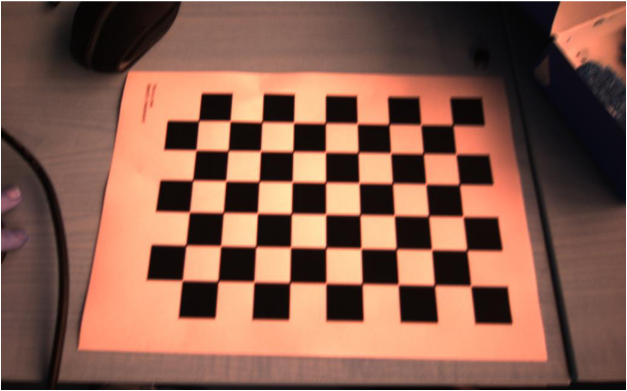
\includegraphics[width=1\linewidth]{pictures//vorkal.png}
          \caption{Bild vor der Kalibrierung}
          \label{fig:vorkal}  
        \end{minipage}
        \hspace{.1\linewidth}
        \begin{minipage}[b]{.4\linewidth}
          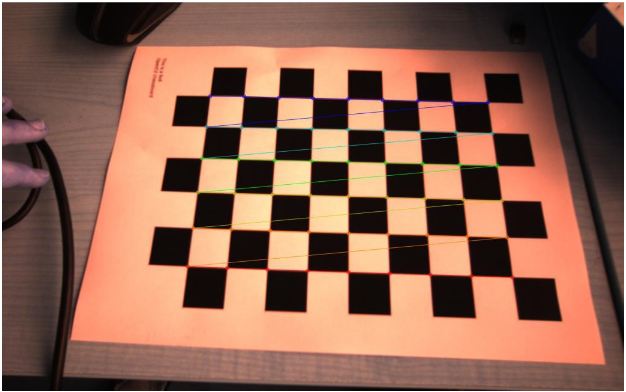
\includegraphics[width=1\linewidth]{pictures//nachkal.png}
          \caption{Bild nach der Kalibrierung}
          \label{fig:nachkal}  
        \end{minipage}
    \end{center}
    
\end{figure}

Im weiteren Verlauf des Praktikums traten erhebliche Ungenauigkeiten in der Positionsbestimmung auf, die die Qualität der Lokalisierungsergebnisse beeinträchtigten. Es wurde die Hypothese aufgestellt, dass die Ursache hierfür in den unzureichend bestimmten Parametern der Kameramatrix und einer möglicherweise fehlerhaften Kalibrierung lag. Zur Verifizierung dieser Annahme wurden daraufhin verschiedene Skripte zur Bestimmung der Kameramatrix und der Verzerrungskoeffizienten getestet. Trotz des Einsatzes mehrerer Kalibrierungsmethoden erwiesen sich die Ergebnisse als unzureichend, da sie keine nennenswerte Verbesserung der Genauigkeit erzielten und sogar merklich ungenauer waren als die ursprünglich ermittelten Werte mithilfe von OpenCV.

Da alternative Kalibrierungsverfahren keine zufriedenstellenden Resultate lieferten, wurde entschieden, die Kameraparameter direkt aus dem Datenblatt der verwendeten Kamera zu entnehmen und die intrinsische Kameramatrix manuell zu befüllen. Die Verzerrungskoeffizienten konnten auf null gesetzt werden, da die eingesetzten Kameras werkseitig bereits entzerrte Bilder lieferten. Durch diese Anpassung wurde die Basis für eine präzisere und verlässlichere Positionsbestimmung geschaffen, was die Qualität der weiteren Experimente im Praktikum erheblich verbesserte.
\newpage

\section{Lösungsansätze}

Im Rahmen des Projekts werden drei U3-3560XLE-C-HQ Rev.1.1 Kameras der Firma IDS Imaging eingesetzt, einem deutschen Unternehmen, das sich auf Industriekameras spezialisiert hat. Diese Kameras sind an einem lokalen Rechner angeschlossen, auf dem Ubuntu 20.04 (Focal Fossa) und ROS Noetic laufen.Beide Versionen verfügen über einen Long-Term-Support bis Mai 2025. Da diese Supportdauer für ein langfristiges Projekt jedoch begrenzt ist und die Software danach keine Sicherheitsupdates oder Wartungspatches mehr erhalten wird, ist diese Lösung nicht wirklich zukunftssicher. Für eine langfristige Nutzung wird daher die Einführung von ROS2 Humble auf Ubuntu 22.04 angestrebt, das mit seinem LTS bis 2027 eine stabilere Basis für die nächsten Jahre bietet. 

Da einige bestehende Anwendungen auf dem System speziell auf Ubuntu 20.04 und ROS Noetic angewiesen sind, wäre ein vollständiges Upgrade auf Ubuntu 22.04 mit ROS2 Humble mit erheblichen Anpassungen verbunden. Alle bestehenden ROS1-Anwendungen müssten auf ROS2 migriert werden, was einen erheblichen Aufwand darstellen würde. Um diesen Aufwand zu vermeiden und dennoch die Vorteile von ROS2 Humble auf dem aktuellen System zu nutzen, werden Docker-Container mit einem Ubuntu 22.04-Image eingerichtet, auf denen ROS2 Humble betrieben wird. 

Ein wesentlicher Nachteil der Verwendung von Docker-Containern ist jedoch die fehlende grafische Benutzeroberfläche (GUI), sodass die Steuerung ausschließlich über Terminal-Befehle oder vordefinierte Skripte erfolgt. Da jedoch eine Visualisierung in RViz erforderlich ist, muss eine Lösung gefunden werden, um die Kommunikation zwischen den ROS1- und ROS2-Knoten zu gewährleisten. Diese Kommunikation wird standardmäßig nicht unterstützt, da ROS1 und ROS2 auf unterschiedlichen Kommunikationsprotokollen basieren.

Zur Lösung dieses Problems wird die ROS2-Distribution Foxy verwendet, die zwar keinen Support mehr erhält, jedoch auf Ubuntu 20.04 installiert werden kann. Es existieren zudem bereits GitHub-Repositories, die die Kommunikation zwischen ROS2 und ROS1 ermöglichen. Mithilfe dieser „Bridge“-Lösung kann ROS2 Foxy mit ROS2 Humble kommunizieren und Nachrichten nahtlos an ROS Noetic weitergeben. Dies ermöglicht es, die erforderliche Visualisierung und Datenverarbeitung zu realisieren und gleichzeitig die langfristige Unterstützung von ROS2 zu nutzen, ohne die bestehende ROS1-Infrastruktur komplett umstrukturieren zu müssen.

\newpage

\subsection{1. Lösungsansatz}

\begin{figure}[htb]
    \centering
    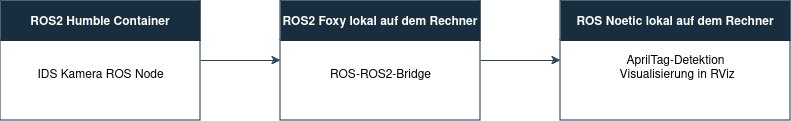
\includegraphics[width=1\linewidth]{pictures/loesungsversuch1.drawio.pdf}
    \caption{Blockdiagramm des 1. Lösungsansatzes}
    \label{fig:ansatz1}
\end{figure}

Im ersten Lösungsansatz wurde die Übertragung der Kameraaufnahmen der IDS-Kameras mithilfe von ROS2 Humble in einem Docker-Container realisiert, während die AprilTag-Detektion in ROS Noetic ausgeführt werden sollte. Dieser Ansatz ermöglichte die Nutzung neuer ROS2-Funktionen zur Bildübertragung, während die bestehende AprilTag-Erkennung in der bewährten ROS Noetic-Umgebung integriert bleiben sollte.

Während der Implementierung traten jedoch mehrere Probleme auf, die die Verwendbarkeit der AprilTag-Detektion beeinträchtigten. Ein zentrales Problem war das Fehlen des `/tf`-Topics, das normalerweise die Koordinaten der erkannten AprilTags im Kamerakoordinatensystem veröffentlicht. Da diese Informationen nicht bereitgestellt wurden, konnten die AprilTags nicht lokalisiert werden, was die Positionsbestimmung unmöglich machte.

Zusätzlich zeigte sich eine inkonsistente Ankunft der Nachrichten für die `Image`- und `Camera Info`-Topics. Obwohl die Kameras mit einer Bildwiederholungsrate von 30 FPS arbeiteten, wurden sowohl die Bilddaten (Image Messages) als auch die Kameraparameter (Camera Info Messages) unregelmäßig und mit stark reduzierter Frequenz empfangen. Dadurch standen die Bild- und Parameterdaten nicht in der erforderlichen Konsistenz und Synchronisation zur Verfügung, was die AprilTag-Detektion für den Anwendungsfall unbrauchbar gemacht hätte.

Nach längerer Fehlersuche wurde die Ursache dieser Probleme in der AprilTag-Detektion innerhalb der ROS Noetic-Umgebung vermutet. Bei anderen Anwendungen zeigte die ROS Bridge in Foxy keine vergleichbaren Schwierigkeiten und konnte Nachrichten korrekt zwischen ROS1 und ROS2 übermitteln. Die Unregelmäßigkeiten traten somit vermutlich in Verbindung mit der AprilTag-Detektion in Noetic auf.

Aufgrund dieser Herausforderungen wurde ein alternativer Lösungsansatz entwickelt: Die AprilTag-Detektion soll vollständig in ROS2 Humble innerhalb eines Docker-Containers realisiert werden. Dieser Ansatz zielt darauf ab, die Synchronisation der Nachrichten zu verbessern und die Erkennung der AprilTags zu optimieren, ohne von möglichen Inkompatibilitäten oder Einschränkungen in der ROS1-Umgebung betroffen zu sein.

\newpage

\subsection{2. Lösungsansatz}


\begin{figure}[htb]
    \centering
    \includegraphics[width=0.75\linewidth]{pictures/loesungsversuch2.drawio.pdf}
    \caption{Blockdiagramm des 2. Lösungsansatz}
    \label{fig:ansatz2}
\end{figure}


Die Implementierung des neuen Ansatzes zeigte positive Ergebnisse, die zuvor aufgetretene Probleme konnten behoben werden. Insbesondere wurde das /tf-Topic erfolgreich generiert, wodurch die für die Lokalisierung erforderlichen Transformationsdaten bereitgestellt werden konnten. Zudem stimmen nun die Image Messages in Frequenz und Synchronisation mit den Camera Info Messages überein, sodass ein konsistenter und verlässlicher Datenstrom gewährleistet ist. Dies bildet die Grundlage für eine präzise und stabile AprilTag-Detektion und eine verlässliche Positionsbestimmung.

In den nächsten Schritten steht die Transformation der Positionen der erkannten AprilTags in ein Koordinatensystem (KOS) an, das unabhängig vom Kamerakoordinatensystem ist. Diese Transformation ist entscheidend, um eine übergreifende Lokalisierung zu ermöglichen, die auf ein globales oder projektspezifisches KOS bezogen ist.

Ein wesentlicher Schritt ist die Validierung der Genauigkeit des neuen Systems. Diese Validierung ist notwendig, um zu bestimmen, wie stark die berechneten Positionen im Mittelwert von den tatsächlichen Positionen abweichen. Für diesen Vergleich wird die Methode der kleinsten Fehlerquadrate angewendet. Dabei wird der Unterschied zwischen den geschätzten und den tatsächlichen Werten minimiert, indem die Quadrate der Fehler summiert und die Summe auf ein Minimum reduziert wird. Auf diese Weise lässt sich quantitativ erfassen, wie präzise die Positionsbestimmung ist, und es wird möglich, potenzielle Abweichungen systematisch zu identifizieren und zu analysieren.

Abschließend ist es notwendig, die extrinsischen Kameraparameter zu bestimmen, die zur präzisen Lokalisierung der Kameras im Raum erforderlich sind. Die Kenntnis dieser Parameter ist wesentlich, um die Position und Ausrichtung der Kameras relativ zueinander und zu einem definierten Ursprung zu spezifizieren. Die Bestimmung der extrinsischen Parameter wird voraussichtlich eine sorgfältige Kalibrierung umfassen, um eine verlässliche, raumbezogene Positionsermittlung zu gewährleisten.

\newpage
\section{Konzeptionierung der Lokalisierung}


\subsection{Auswahl einer geeigneten Tag-Family}

AprilTags sind visuelle Marker, die als Referenzsysteme für präzise Positions- und Orientierungsbestimmungen dienen. Sie bestehen aus einem festen Koordinatensystem und einem einzigartigen Muster, das in einer spezifischen Datenbank gespeichert und einer eindeutigen ID zugeordnet ist. Dies ermöglicht die Unterscheidung zwischen verschiedenen Tags in der Anwendung und trägt zur Identifizierung spezifischer Marker bei, was besonders in Robotik und autonomen Fahrsystemen von hoher Relevanz ist. Da AprilTags Open-Source-basiert sind, kann jeder Nutzer seine eigene Tag-Familie erstellen, was zu einer fortlaufenden Erweiterung und Anpassung der verfügbaren Tags führt. Trotz dieser Dynamik existieren einige etablierte Tag-Families, die auf unterschiedliche Anwendungsbedürfnisse zugeschnitten sind. 

Zu den wichtigsten AprilTag-Familien gehören 25h9, 16h5 und 36h11, die jeweils spezifische Eigenschaften besitzen, die sie für unterschiedliche Anwendungen prädestinieren. Die Tag-Familie 25h9 verwendet 25 Bits und weist eine Hamming-Distanz von 9 auf. Dies bedeutet, dass die Tags dieser Familie im Vergleich zu solchen mit höheren Bit-Längen und Hamming-Distanzen weniger robust gegenüber Fehlern sind. Der Vorteil dieser Konfiguration liegt jedoch in der größeren Anzahl möglicher, eindeutig unterscheidbarer Tags, die generiert werden können. Dadurch eignet sich die 25h9-Familie besonders gut für Einsatzbereiche, in denen eine Vielzahl von Tags auf engem Raum platziert werden muss und dennoch zuverlässig erkannt werden soll – beispielsweise in Umgebungen mit hoher Tag-Dichte oder bei Anwendungen, die kleine Markierungen erfordern.

Die Tag-Familie 16h5 verwendet lediglich 16 Bits und eine Hamming-Distanz von 5, was sie zur kleinsten und am wenigsten robusten der drei genannten Familien macht. Aufgrund der begrenzten Bit-Anzahl ist die Fehlertoleranz gering, und die Anzahl eindeutiger Tags ist begrenzt. Dennoch sind die Tags aufgrund ihrer geringen Größe besonders geeignet für Anwendungen, in denen Platzmangel herrscht und die Erkennung aus kurzer Distanz erfolgt. Allerdings zeigt sich diese Familie empfindlicher gegenüber ungünstigen Umgebungsbedingungen, was sie weniger geeignet für Situationen macht, in denen die Tags teilweise verdeckt oder aus größerer Entfernung erfasst werden müssen.

Die Tag-Familie 36h11 stellt hingegen die robusteste und vielseitigste der drei genannten Familien dar. Sie verwendet 36 Bits und eine Hamming-Distanz von 11, wodurch eine hohe Fehlertoleranz erreicht wird. Dies ermöglicht die zuverlässige Erkennung auch unter schwierigen Bedingungen, beispielsweise wenn Tags teilweise verdeckt sind oder Störungen auftreten. Die Kombination aus hoher Fehlertoleranz und der großen Anzahl möglicher eindeutiger Tags macht die 36h11-Familie zu einer der weitverbreitetsten und flexibel einsetzbaren Optionen, insbesondere in anspruchsvollen und kritischen Anwendungsbereichen.

Für die Anforderungen unserer Anwendung erweist sich die Tag-Family 36h11 als besonders geeignet. Da es erforderlich ist, dass die Tags auch bei komplexen und dynamischen Szenarien klar voneinander unterscheidbar sind – etwa wenn mehrere Fahrzeuge oder Tags an demselben Fahrzeug gleichzeitig erkannt werden müssen – erfüllt 36h11 diese Voraussetzung durch ihre optimierte Balance aus Erkennungsdichte und Fehlerkorrektur. Außerdem ist die hohe Fehlerkorrektur von Vorteil, da die AprilTags in vielen Fällen nicht in optimaler Ausrichtung zur Kamera platziert sind, was die Detektionsgenauigkeit ohne eine leistungsfähige Korrekturfunktion beeinträchtigen könnte. \autoref{fig:rvizpic1} zeigt eine Szene in RViz 2, ein 3D-Visualisierungstool von ROS 2, wie ein Apriltag und die Ausrichtung seines Koordinatensystems, sowie der Translationsvektor zur Kamera dargestellt wird.

\begin{figure}[htb]
    \centering
    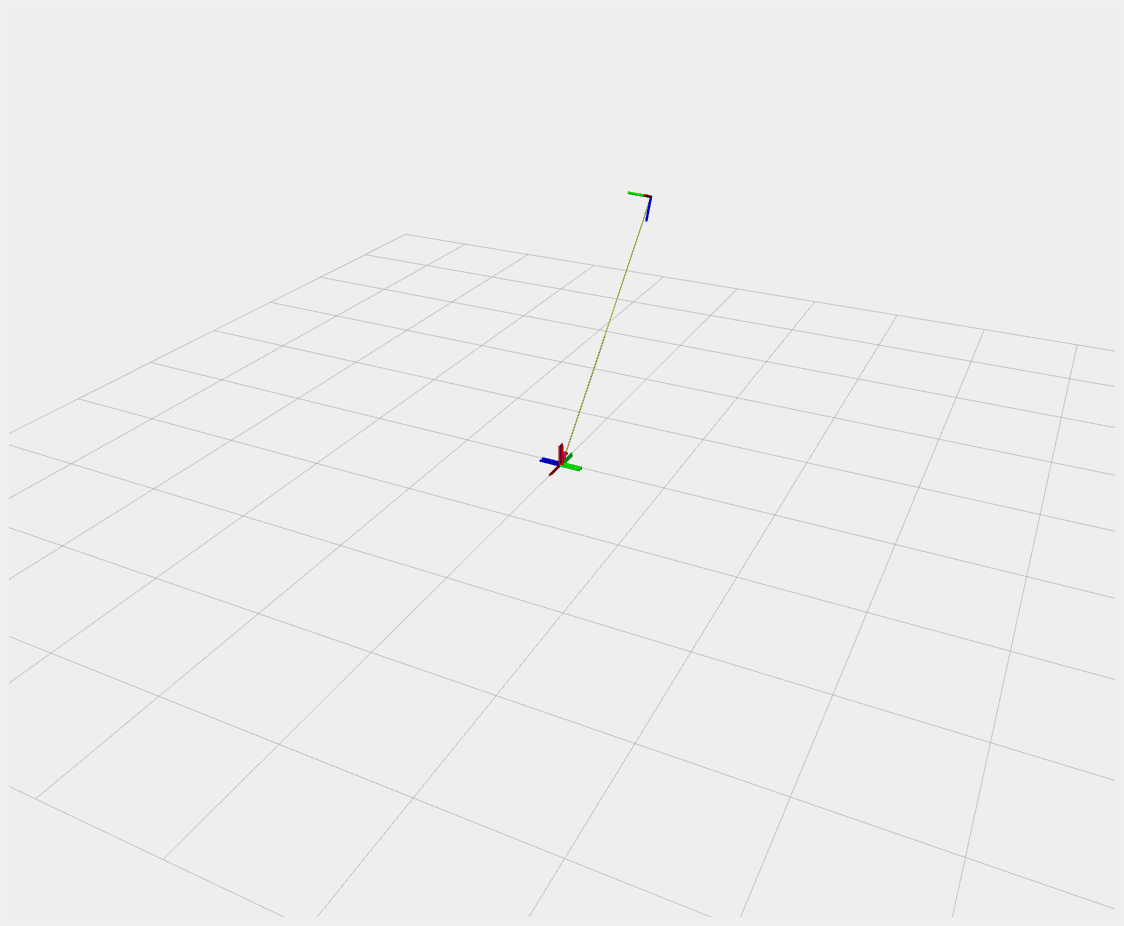
\includegraphics[width=0.5\linewidth]{pictures//rviz picture.png}
    \caption{Darstellung der Position des AprilTags zur Kamera in RViz2}
    \label{fig:rvizpic1}
\end{figure}


\subsection{Berechnung der Position des AprilTags von 2D-Bildebene zum 3D-Weltkoordinatensystem}

In der AprilTag-Lokalisierung für Anwendungen in autonomen Fahrzeugen spielen das Bildkoordinatensystem, das Kamerakoordinatensystem und das Weltkoordinatensystem eine zentrale Rolle. Diese Koordinatensysteme ermöglichen die präzise Bestimmung der Position und Orientierung von AprilTags, die als Referenzpunkte für die Fahrzeugnavigation und -steuerung dienen können.


Das Bildkoordinatensystem ist das 2D-Koordinatensystem, das durch die Pixel des Kamerabildes definiert wird. Hierbei hat jeder Pixelpunkt eine Position \((u, v, w)\), die seine Lage innerhalb des Bildes beschreibt. In den meisten Bildverarbeitungsframeworks liegt der Ursprung dieses Systems in der oberen linken Bildecke. In diesem Fall liegt jedoch im optischen Zentrum wobei die \( u \)-Achse horizontal nach rechts und die \( v \)-Achse vertikal nach unten verläuft. Die Koordinaten werden in Pixeln angegeben und beschreiben die Position eines Punktes nur innerhalb der 2D-Projektion. Im Rahmen der AprilTag-Detektion wird das Tag im Bildkoordinatensystem lokalisiert, indem die Eckpunkte des Tags durch eine ROS-Node identifiziert werden. Dies liefert zunächst nur die 2D-Position der Tags im Bild, wodurch noch keine Rückschlüsse auf deren räumliche Position möglich sind. Um jedoch eine Tiefeninformation und eine genaue Positionierung im Raum zu erlangen, müssen die Bildkoordinaten ins 3D-Kamerakoordinatensystem überführt werden.


Das Kamerakoordinatensystem ist ein dreidimensionales, kartesisches Koordinatensystem, dessen Ursprung am optischen Zentrum der Kamera liegt. In diesem System zeigt die \( z \)-Achse entlang der Blickrichtung der Kamera, während die \( x \)-Achse horizontal und die \( y \)-Achse vertikal verläuft. Die Koordinaten eines Punktes in diesem System, etwa \( (X, Y, Z) \), beschreiben seine Position relativ zur Kamera und geben die räumliche Tiefe an. Um die AprilTags in den Kamerakoordinaten zu lokalisieren, werden die intrinsischen Kameraparameter verwendet, die aus der Kamerakalibrierung stammen und die Transformation der 2D-Bildkoordinaten \((u, v)\) in 3D-Kamerakoordinaten \((X, Y, Z)\) nach \cite{Wang} ermöglichen. Die Kenntnis der Position eines AprilTags im Kamerakoordinatensystem erlaubt es, die Tiefe und Entfernung eines Tags von der Kamera zu bestimmen, was für autonome Fahrzeuge essenziell ist, um eine genaue räumliche Orientierung und Abstandsinformationen zu erhalten.

\begin{equation}
    \begin{pmatrix}
        u \\
        v\\
        w\\
    \end{pmatrix} =
    \begin{pmatrix}
         \text{f}_x & 0 & \text{c}_x & 0 \\ 0 & \text{f}_y & \text{c}_y & 0 \\ 0 & 0 & 1 & 0
    \end{pmatrix}
    \begin{pmatrix}
        \text{x}_c \\
        \text{y}_c \\
        \text{z}_c \\
        1
    \end{pmatrix}
\end{equation}


Das Weltkoordinatensystem ist ein übergeordnetes, stationäres Koordinatensystem, das als globales Referenzsystem für die Umgebung des Fahrzeugs dient. Die Koordinaten eines Punktes im Weltkoordinatensystem werden durch \( (X_w, Y_w, Z_w) \) beschrieben und sind unabhängig von der Position und Ausrichtung der Kamera. Um die Position eines AprilTags im Weltkoordinatensystem darzustellen, ist eine Transformation von den Kamerakoordinaten in das Weltkoordinatensystem erforderlich. Diese erfolgt durch eine Rotations- und Translationsmatrix, die die Lage und Orientierung der Kamera relativ zum Weltkoordinatensystem beschreibt. Eine präzise Umrechnung der Kamerakoordinaten ins Weltkoordinatensystem ermöglicht es, das AprilTag als fixen Punkt in einem globalen Kontext darzustellen und die Position des Fahrzeugs unabhängig von der Kameraausrichtung und -position zu bestimmen. Dies ist besonders wichtig für autonome Fahrzeuge, um sich auf ihre Umgebung zu beziehen und ihre eigene Position zu verifizieren, selbst bei mehreren oder sich bewegenden AprilTags.

\begin{equation}
    \begin{pmatrix}
        \text{z}_c \\
        \text{z}_c \\
        \text{z}_c \\
        1
    \end{pmatrix} = \begin{pmatrix}
        \text{r}_{11} & \text{r}_{12} & \text{r}_{13} & \text{t}_x \\
        \text{r}_{21} & \text{r}_{22} & \text{r}_{23} & \text{t}_y \\
        \text{r}_{31} & \text{r}_{23} & \text{r}_{33} & \text{t}_z \\
        0 & 0 & 0 & 1
    \end{pmatrix}
    \begin{pmatrix}
        \text{x}_w \\
        \text{y}_w \\
        \text{z}_w \\
        1
    \end{pmatrix}
\end{equation}

Das Zusammenspiel dieser Koordinatensysteme ermöglicht die präzise Positionierung der AprilTags und unterstützt die räumliche Orientierung des Fahrzeugs in seiner Umgebung. Zunächst wird das AprilTag im Bildkoordinatensystem identifiziert und seine Eckpunkte erfasst. Danach erfolgt eine Transformation ins Kamerakoordinatensystem, welche die Tiefeninformation des Tags liefert. Schließlich wird die Position des AprilTags mithilfe der Rotations- und Translationsmatrix ins Weltkoordinatensystem übertragen, sodass die Position und Orientierung des Tags in einem globalen Rahmen genutzt werden kann. Damit erhält das Fahrzeug genaue Informationen über die Position der AprilTags, die als Orientierungspunkte für die sichere und präzise Navigation verwendet werden können. Um die Transformation von Bildebene in das Weltkoordinaten in einem Schritt zu durchlaufen, können die intrinsiche und extrinsische Kameramatrix zur Projetionsmatrix $\text{P}$ zusammengefasst werden. 

\begin{equation}
    \text{P} = \begin{pmatrix}
         \text{f}_x & 0 & \text{c}_x \\ 0 & \text{f}_y & \text{c}_y \\ 0 & 0 & 1 
    \end{pmatrix}
    \begin{pmatrix}
        \text{r}_{11} & \text{r}_{12} & \text{r}_{13} & \text{t}_x \\
        \text{r}_{21} & \text{r}_{22} & \text{r}_{23} & \text{t}_y \\
        \text{r}_{31} & \text{r}_{23} & \text{r}_{33} & \text{t}_z \\
        0 & 0 & 0 & 1
    \end{pmatrix}
    = 
   \begin{pmatrix}
        \text{p}_{11} & \text{p}_{12} & \text{p}_{13} & \text{p}_{14} \\
        \text{p}_{21} & \text{p}_{22} & \text{p}_{23} & \text{p}_{24} \\
        \text{p}_{31} & \text{p}_{23} & \text{p}_{33} & \text{p}_{34} \\
        0 & 0 & 0 & 1
    \end{pmatrix} 
\end{equation}

\newpage
Damit ergibt sich:

\begin{equation}
    \begin{pmatrix}
        u \\
        v\\
        w\\
    \end{pmatrix} = \begin{pmatrix}
        \text{p}_{11} & \text{p}_{12} & \text{p}_{13} & \text{p}_{14} \\
        \text{p}_{21} & \text{p}_{22} & \text{p}_{23} & \text{p}_{24} \\
        \text{p}_{31} & \text{p}_{23} & \text{p}_{33} & \text{p}_{34} \\
        0 & 0 & 0 & 1
    \end{pmatrix}  
    \begin{pmatrix}
        \text{x}_w \\
        \text{y}_w \\
        \text{z}_w \\
        1
    \end{pmatrix}.
\end{equation}

Bisher wurde dargelegt, wie Transformationen vom Weltkoordinatensystem zurück in die Bildebene vorgenommen werden. Um jedoch die Weltkoordinaten eines gegebenen Bildpunktes zu bestimmen, müssen die zugrundeliegenden Gleichungen zunächst ausformuliert werden. In der AprilTag-Lokalisierung werden die einzelnen Tags durch ihre vier Eckpunkte erfasst. Hierdurch ergibt sich ein überbestimmtes Gleichungssystem, da mehr als die minimal benötigten Punkte zur Berechnung der Position vorliegen. 

\begin{align}
    u &= p_{11} \cdot x_w + p_{12} \cdot y_w + p_{13} \cdot z_w + p_{14} \\
    v &= p_{21} \cdot x_w + p_{22} \cdot y_w + p_{23} \cdot z_w + p_{24} \\
    w &= p_{31} \cdot x_w + p_{32} \cdot y_w + p_{33} \cdot z_w + p_{34}
\end{align}

Um diese nach den Weltkoordinaten \(x_w\), \(y_w\) und \(z_w\) aufzulösen, teilen wir zunächst die Gleichungen für \(u\) und \(v\) jeweils durch \(w\), um die normierten Koordinaten \(\tilde{u} = \frac{u}{w}\) und \(\tilde{v} = \frac{v}{w}\) zu erhalten.

\begin{align}
    \tilde{u} &= \frac{p_{11} \cdot x_w + p_{12} \cdot y_w + p_{13} \cdot z_w + p_{14}}{p_{31} \cdot x_w + p_{32} \cdot y_w + p_{33} \cdot z_w + p_{34}} \\
    \tilde{v} &= \frac{p_{21} \cdot x_w + p_{22} \cdot y_w + p_{23} \cdot z_w + p_{24}}{p_{31} \cdot x_w + p_{32} \cdot y_w + p_{33} \cdot z_w + p_{34}}
\end{align}

Eine gängige Methode zur Schätzung der Position ist in diesem Kontext die Methode der kleinsten Quadrate, die durch Minimierung der quadrierten Abweichungen eine optimale Lösung liefert.

Da bei der AprilTag-Detektion das Kamerakoordinatensystem als Referenz verwendet wird, werden die berechneten Weltkoordinaten nur in diesem Koordinatensystem angegeben. Für die Darstellung von Rotationen werden Quaternionen verwendet, da diese gegenüber den klassisch verwendeten Rotationsmatrizen mit Euler-Winkeln wesentliche Vorteile aufweisen. Zum einen ermöglichen Quaternionen eine einfache Berechnung der Rotation, da sie keine einzelnen Rotationsmatrizen für jede Achse erfordern, wie dies bei Euler-Winkeln oder Drehmatrizen der Fall ist. Dies führt zu einer höheren Effizienz, was insbesondere in Echtzeitanwendungen vorteilhaft ist. Zum anderen verhindern Quaternionen das Auftreten eines Gimbal Locks. Der Gimbal Lock ist ein Problem, das bei der Darstellung und Berechnung von Rotationen in dreidimensionalen Koordinatensystemen auftreten kann, wenn diese mit Euler-Winkeln beschrieben werden. Euler-Winkel sind eine Methode, um die Rotation eines Objekts durch drei aufeinanderfolgende Drehungen um verschiedene Achsen darzustellen. Diese Drehungen sind jedoch anfällig für den Gimbal Lock, wenn zwei der drei Rotationsachsen zusammenfallen oder parallel werden.

Zur Definition des Weltkoordinatensystems wird ein sogenannter Null-AprilTag als Anfangspunkt gesetzt. Dieser Tag dient als fester Referenzpunkt, von dem die Position und Rotation relativ zur Kamera gemessen werden können. Durch diese Ausgangsreferenz lassen sich dann die Translation und Rotation der Kamera in Bezug auf den Null-AprilTag bestimmen. Mit dieser Information kann die Position des Kamerakoordinatensystems in das Koordinatensystem des Null-AprilTags transformiert werden, sodass eine kohärente Darstellung der Weltkoordinaten gegeben ist.

Ein Quaternion \( q \) für die Rotation kann in der Form \( q = (w, x, y, z) \) geschrieben werden, wobei \( w \) der Skalarteil und \( (x, y, z) \) der vektorielle Teil ist. Somit erfolgt eine Punktdrehung mithilfe der Quaternion folglich:

\begin{equation}
    \vec{v_\text{neu}} = q \cdot \vec{v} \cdot q^{-1}
\end{equation}

Da wir jedoch nicht im Basisisystem, also dem Kamerakoordinatensystem drehen möchten, sondern das Kamerasystem deckungsgleich mit dem Koordinatensystems des 0-Apriltags drehen möchten müssen wir die Multiplikation mit der Inversen der Quaternion berginnen. Die Umwandlung der Koordinaten eines Vektors von Kamerakoordinaten in Weltkoordinaten, also dem 0-Apriltag, unter Verwendung von Quaternionen erfolgt durch folgende Gleichung:

\begin{equation}
    \vec{v_{w}} = q^{-1} \cdot \vec{v_{c}} \cdot q + \vec{t_{K}}
    \label{eq:17}.
\end{equation}


Hierbei ist \( q^{-1} \) die Inverse der Quaternionen \( q \) und \(\vec{t_{K}}\) der Translationsvektor von Kamera zu 0-Apriltag.

Die Verwendung mehrerer Kameras erfordert eine dynamische Betrachtung der Translationen, da es nicht ausreichend ist, die Translation einer einzelnen Kamera zum Null-AprilTag statisch im Skript zu hinterlegen. Die extrinsischen Parameter sind von zentraler Bedeutung, da sie die relative Lage der einzelnen Kameras zueinander beschreiben und daher berechnet werden müssen. In \autoref{fig:extrpara} wird angenommen, dass nur eine Kamera den Null-AprilTag erkennt. Allerdings sehen alle drei Kameras einen zweiten AprilTag, wodurch die Vektoren zwischen den Kameras anhand der Vektoren zum gemeinsam detektierten AprilTag bestimmt werden können.

\begin{figure}[htb]
    \centering
    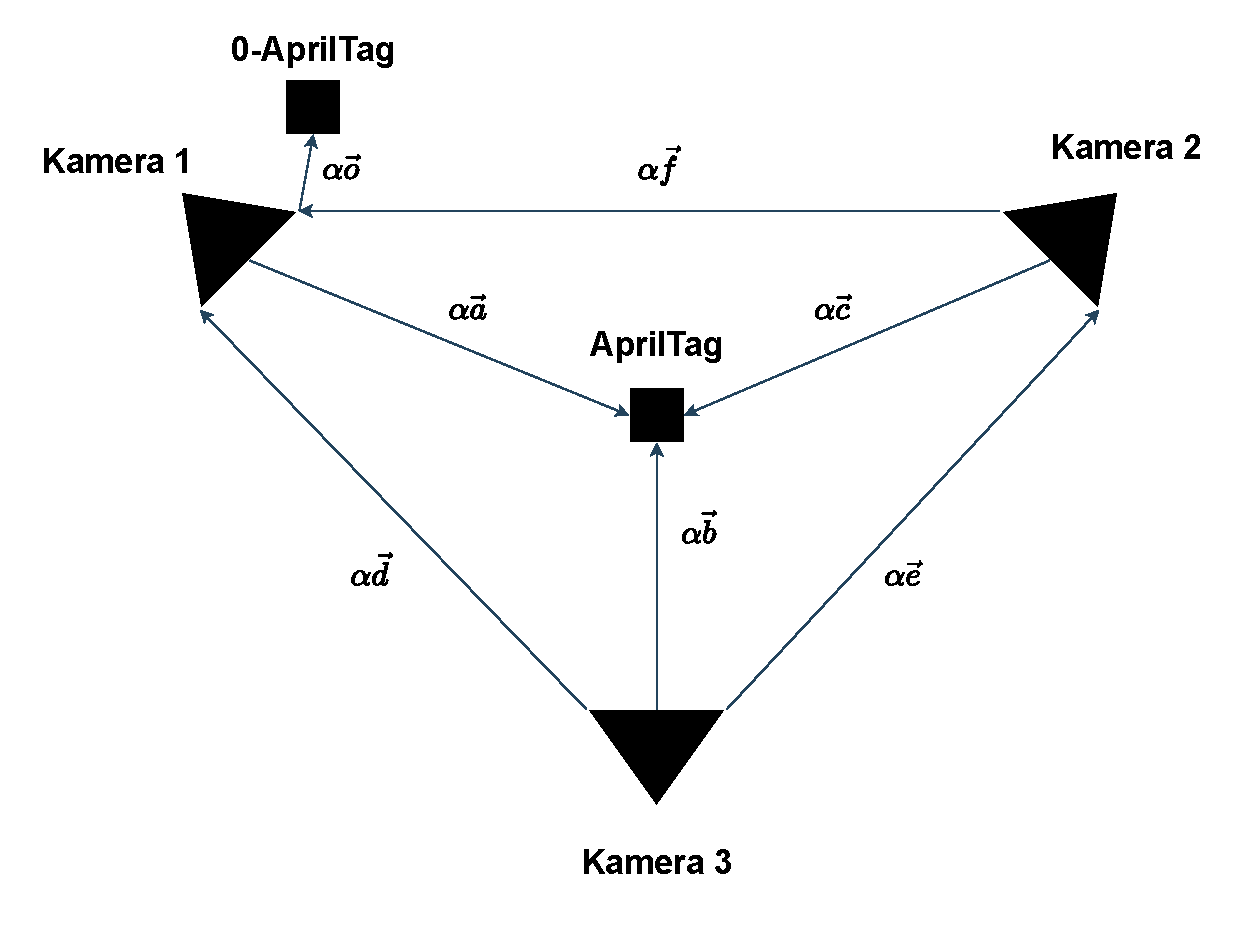
\includegraphics[width=0.5\linewidth]{pictures/extrpara.drawio-1.pdf}
    \caption{Vektorenbeziehungen zwischen Kameras und AprilTags}
    \label{fig:extrpara}
\end{figure}

\FloatBarrier

Auf den Streckungsfaktor \(\alpha\) werde ich im 5. Kapitel näher eingehen. Zunächst stellen wir die Vektorbeziehungen auf, welche wir benötigen um die Translation \(\mathbf{T}_{K1...3}\) von den Kameras zum 0-AprilTag zu berechnen. Damit ergeben sich damit folgende Gleichungen aus \autoref{fig:extrpara}:

\begin{align}
    \alpha \vec{f} = \alpha \vec{c} - \alpha \vec{a}\\\alpha \vec{d} = \alpha \vec{b} - \alpha \vec{a}
\end{align}
. 

Damit konnten wir von Kamera 2 und 3 zurück auf Kamera 1 schließen, von der wir nun die Translation zum 0-AprilTag der einzelnen Kameras bestimmen können, indem wir \(\alpha\vec{o}\), den Vektor von Kamera 1 zum 0-AprilTag mit in die Gleichungen einbeziehen:

\begin{align}
    \mathbf{T}_{K1} = \alpha \vec{o}\\\mathbf{T}_{K2} = \alpha \vec{f} + \alpha \vec{o}\\\mathbf{T}_{K3} = \alpha \vec{d} + \alpha \vec{o}  
\end{align}
.
Es ist nicht zwingend erforderlich, dass die zuvor erwähnte Konstellation erreicht wird. Solange es möglich ist, einen Vektor von jeder einzelnen Kamera zurück zum Null-AprilTag zu berechnen, können die extrinsischen Parameter ermittelt werden, wenn auch mit anderen Gleichungen. Dadurch wird es möglich, die spezifischen Parameter für jede Kamera im Skript zu hinterlegen, was eine Transformation der Koordinaten vom Kamerakoordinatensystem in das Koordinatensystem des Null-AprilTags ermöglicht.

Das /tf-Topic hinterlegt, in der TFMessage, welche Kamera den AprilTag detektiert, und wird als Frame ID wiedergegeben. Dies ermöglicht eine informierte Entscheidung darüber, welche Parameter für den Translationsanteil in \cref{eq:17} verwendet werden. Diese Herangehensweise gewährleistet eine präzise Berechnung der Positionen und eine verbesserte Integration der Kameradaten in das Gesamtsystem.

\begin{figure}[htb]
    \centering
    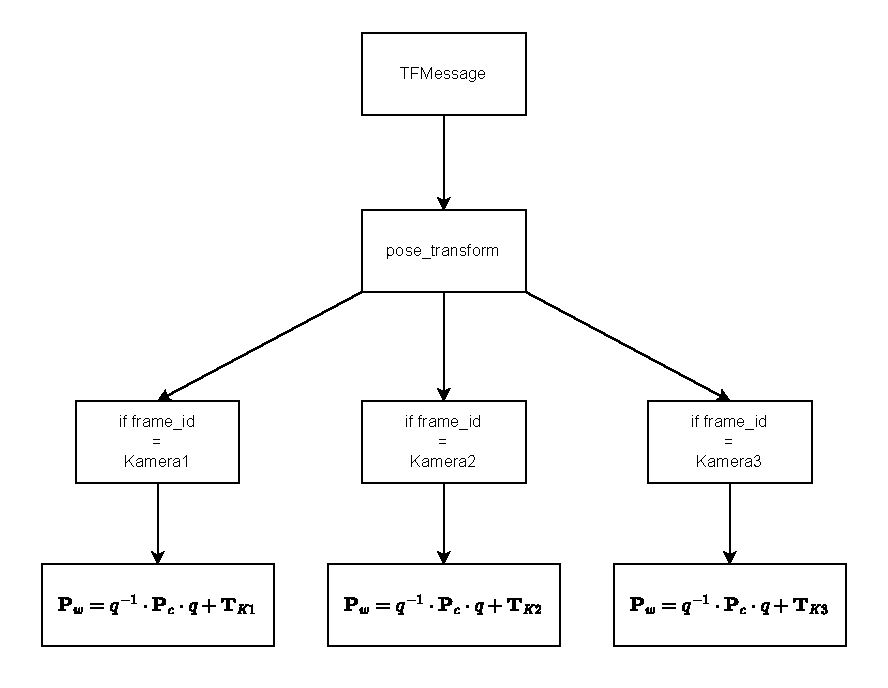
\includegraphics[width=0.5\linewidth]{pictures/papextr.drawio.pdf}
    \caption{Blockdiagramm der Verzweigung für die Auswahl der richtigen Translationskomponente}
    \label{fig:papextr}
\end{figure}

\newpage

\subsection{Genauigkeit der Lokalisierung}

In der Auswertung der AprilTag-Detektionsdaten spielt der Faktor \( \alpha \) aus der Abbildung eine zentrale Rolle. Dieser Faktor beschreibt die mittlere Abweichung zwischen den durch die AprilTag-Erkennung erfassten Messdaten und den tatsächlichen, realen Werten. Damit wird \( \alpha \) als Skalierungsfaktor der Vektoren verwendet, um systematische Abweichungen in den Detektionsdaten zu identifizieren und zu quantifizieren.

Zur Bestimmung von \( \alpha \) wird die Methode der kleinsten Fehlerquadrate angewendet. Durch dieses Verfahren lassen sich die Differenzen zwischen den gemessenen und den tatsächlichen Werten minimieren, indem \( \alpha \) so angepasst wird, dass die Summe der quadrierten Abweichungen möglichst gering ist. Diese Methode bietet eine optimale Anpassung des Faktors und erlaubt eine präzise Korrektur der AprilTag-Detektionsdaten. Die Berechnung von \( \alpha \) ist somit essenziell für die Verbesserung der Genauigkeit der Detektion und trägt zur Zuverlässigkeit des Systems bei.

Da die Messwerte aus der AprilTag Detektion \(\vec{m_i}\) und die realen Werte \(\vec{r_i}\) beide Vektoren sind, ist es notwendig ihre euklidische Norm nach \cite{kuhnel2011matrizen} zu berechnen, um einen skalaren Wert zu erhalten.
    
Indem wir die euklidische Norm in die Gleichung für die kleinsten Fehlerquadrate einfügen, können wir nach \cite{kauffmanndesign} mit der Berechnung für einen optimierten Streckungsfaktor \(\alpha\) beginnen.

\begin{equation} \label{sum}
    f(\alpha) =  \sum_{ i=1 }^{ n }(|\vec{r_i} - \vec{m_i} \cdot \alpha|)^2 
\end{equation}

\autoref{sum} stellt nun unseren mittleren Fehler dar. Nun ist ein \(\alpha\) zu ermitteln, welches die die erste Ableitung Null werden lässt.

\begin{equation}
    0 = f'(\alpha) = \frac{\text{d}f}{\text{d}\alpha} f(\alpha) = 2\left(\alpha \sum_{i=1}^{n} \|\vec{m_i}\|^2 - \sum_{i=1}^{n} (\vec{r_i} \cdot \vec{m_i})\right)
\end{equation}

Nach Ausmultiplikation und umstellen nach \(\alpha\) ergibt sich:

\begin{equation}
    \alpha = \sum_{i=1}^{n} \frac{ (\vec{r_i} \cdot \vec{m_i})}{ \|\vec{m_i}\|^2}
\end{equation}

Als optimaler Wert für den Skalierungsfaktor \(\alpha\) wurde \(\alpha = 1.637362\) berechnet. Mit diesem Wert ergab sich schließlich eine Standardabweichung der Messdaten von \(6,35 \, \text{cm}\) in \(X\)-Richtung und \(5,37 \, \text{cm}\) in \(Y\)-Richtung. Diese Abweichungen zeigen die Genauigkeit der AprilTag-Detektion und bieten eine verlässliche Grundlage für die Transformation der ermittelten Kamerakoordinaten in das Weltkoordinatensystem. Die Genauigkeitsanalyse bestätigt die Eignung des gewählten Skalierungsfaktors für die angestrebte Präzision der Positionsbestimmung im System.

\begin{figure}[htb]
    \centering
    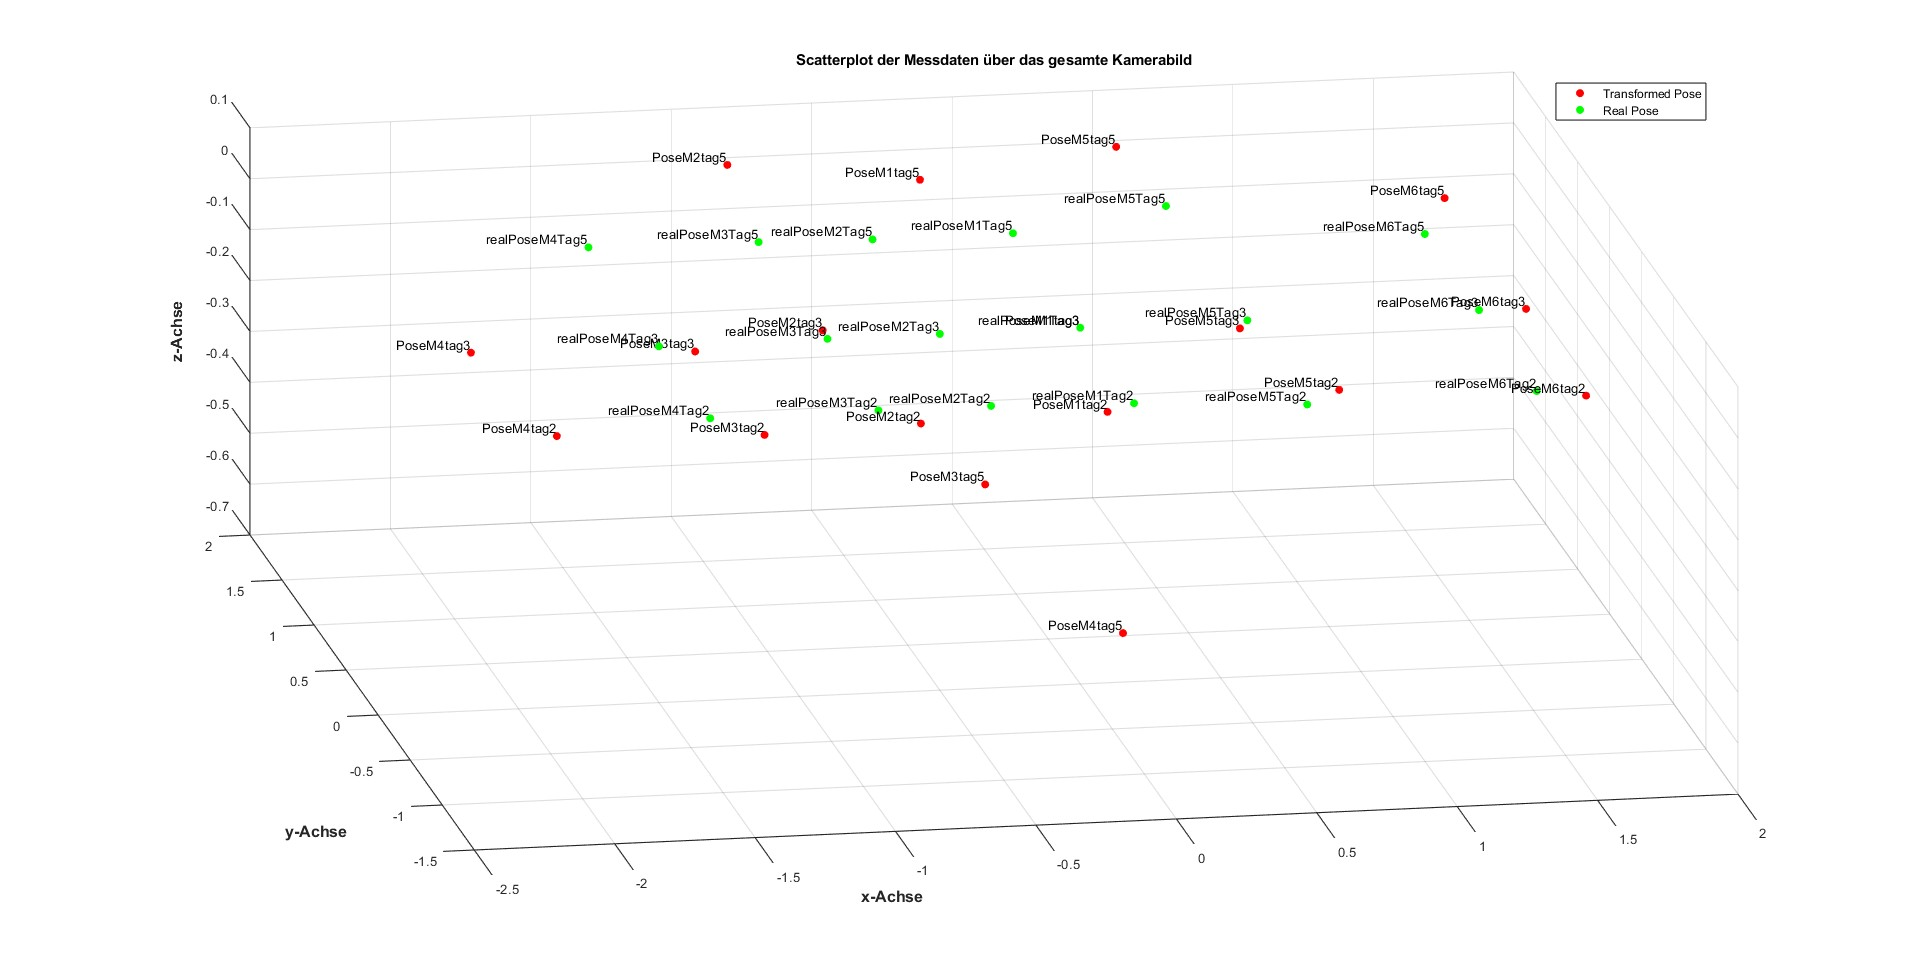
\includegraphics[width=1\linewidth]{pictures/Real_Pose_vs_Transformed_Pose_wiout_alpha.jpg}
    \caption{Scatterplot der unkorrigierten Messwerte}
    \label{fig:plotwoutalpha}
\end{figure}

\begin{figure}[hb]
    \centering
    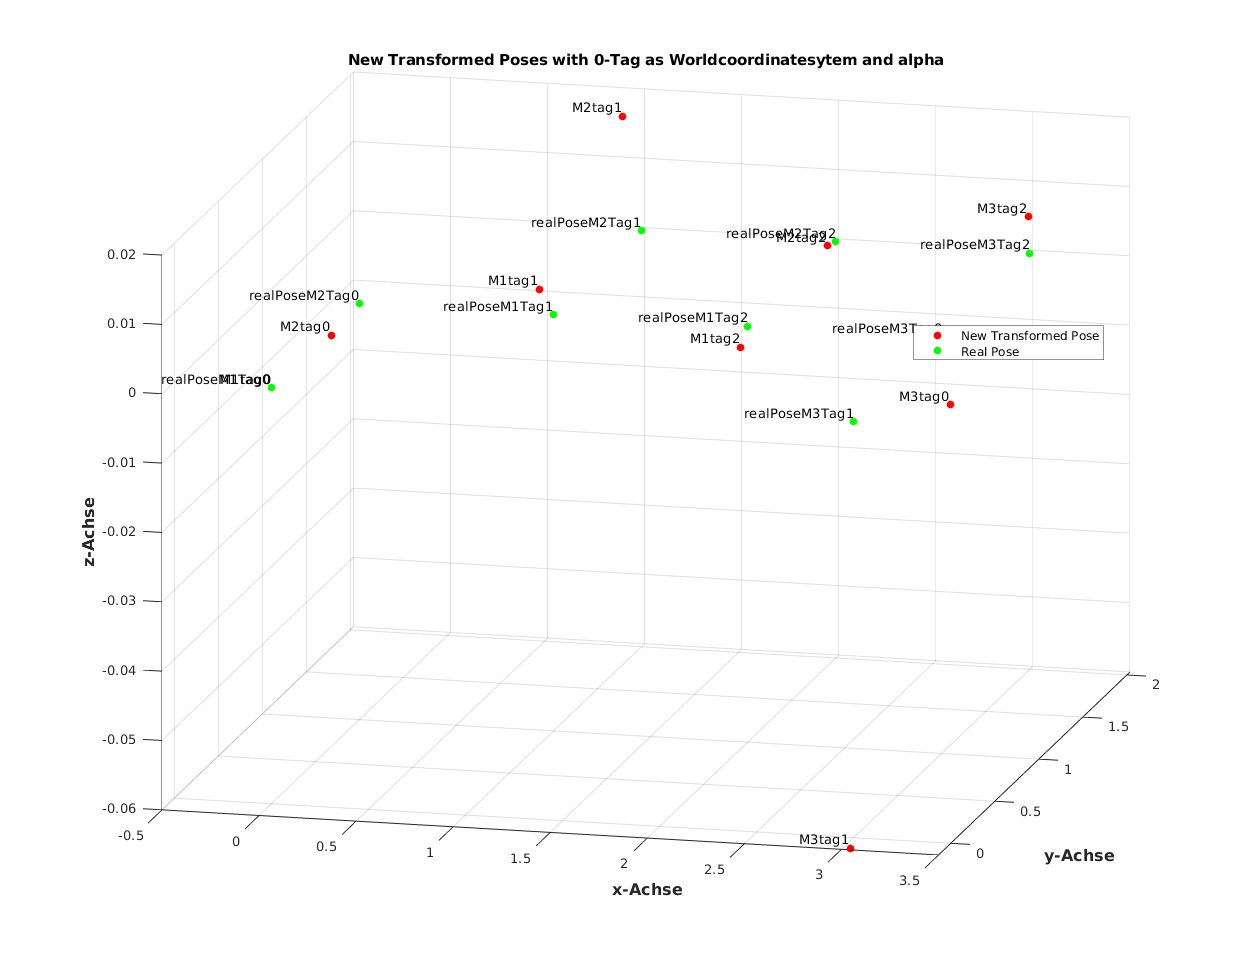
\includegraphics[width=1\linewidth]{pictures/nposewalpha.png}
    \caption{Scatterplot der korrigierten Messwerte}
    \label{fig:plotwalpha}
\end{figure}

\FloatBarrier

\newpage

\section{Resümee}

Im Rahmen dieses Praktikums wurde eine Methode zur Lokalisierung eines 1:8 Fahrzeugmodells entwickelt und getestet. Zu Beginn erfolgten eine umfassende Literaturrecherche und die Einarbeitung in die grundlegenden Konzepte der Bildverarbeitung, Robotik und Systemintegration. Diese Schritte legten die theoretische Basis für die Anwendung der AprilTag Detektion zur Fahrzeuglokalisierung. Das Ergebnis der praktischen Tests zeigte, dass die AprilTag Detektion eine vergleichsweise einfache und effektive Möglichkeit bietet, Positionen zu bestimmen, solange durchschnittliche Abweichungen von 5 bis 6 cm tolerierbar sind.

Die Tests wurden durchgeführt, indem die Messwerte aus der AprilTag Detektion systematisch aufgezeichnet und ausgewertet wurden, während sich die Markierungen stufenweise von der Kamera entfernten. Dabei konnte festgestellt werden, dass die Erkennungsrate mit zunehmendem Abstand abnimmt, bis die AprilTags letztlich nicht mehr detektiert wurden.

Dieses Praktikum an der WHZ bot mir die wertvolle Gelegenheit, eigenständig ein Thema zu bearbeiten, das außerhalb der in der Kraftfahrzeugtechnik behandelten Module liegt, und mich an einem anspruchsvollen Projekt zu erproben. Mein Studium und die Vertiefung in Kraftfahrzeugmechatronik ermöglichten es mir zudem, durch Wahlmodule die Grundlagen in Python und Matlab zu erlernen und diese Kenntnisse im Rahmen des Praktikums weiter zu vertiefen. Ich möchte mich herzlich bei Prof. Dr.-Ing. Rick Voßwinkel und den wissenschaftlichen Mitarbeitern Felix Krabbes, Jan-Philip Rehbein und Philipp Münst bedanken. Sie haben mir nicht nur bei der Bearbeitung dieser anspruchsvollen Aufgabe zur Seite gestanden, sondern mir auch eine inspirierende und förderliche Arbeitsumgebung zur Verfügung gestellt.

\newpage
\nocite{*}
\printbibliography


\end{document}
